\chapter[Metodologia]{Metodologia}
Este capítulo tem como objetivo apresentar a metodologia utilizada para desenvolvimento do TCC 1, e mostrar o plano base que servirá como guia para o desenvolvimento do TCC 2. A seção \ref{met_pesquisa} apresenta a classificação da metodologia utilizada para o desenvolvimento do trabalho juntamente com o plano metodológico. A seção \ref{met_desenvolvimento} descorre sobre o processo de desenvolvimento utilizado na criação da solução. E por último a seção  \ref{cronograma} apresenta o cronograma utilizado no desenvolvimento do TCC 1 é um cronograma para o TCC 2.
\section{Metodologia de Pesquisa}
\label{met_pesquisa}
Segundo \cite{moresi_metodologia_2003} a pesquisa pode ser entendida como um conjunto de ações que tem como objetivo encontrar um problema, construida através de procedimentos empíricos e sistemáticos. Para Moresi existem quatro classificações básicas para a pesquisa, quanto a sua natureza, sua abordagem, seu objetivo e o meio pelo qual é feita a investigação. A figura \ref{img:met_pesquisa} apresenta em quais características este trabalho se apresenta.
\graphicspath{{figuras/}}
\begin{figure}[h]
\centering
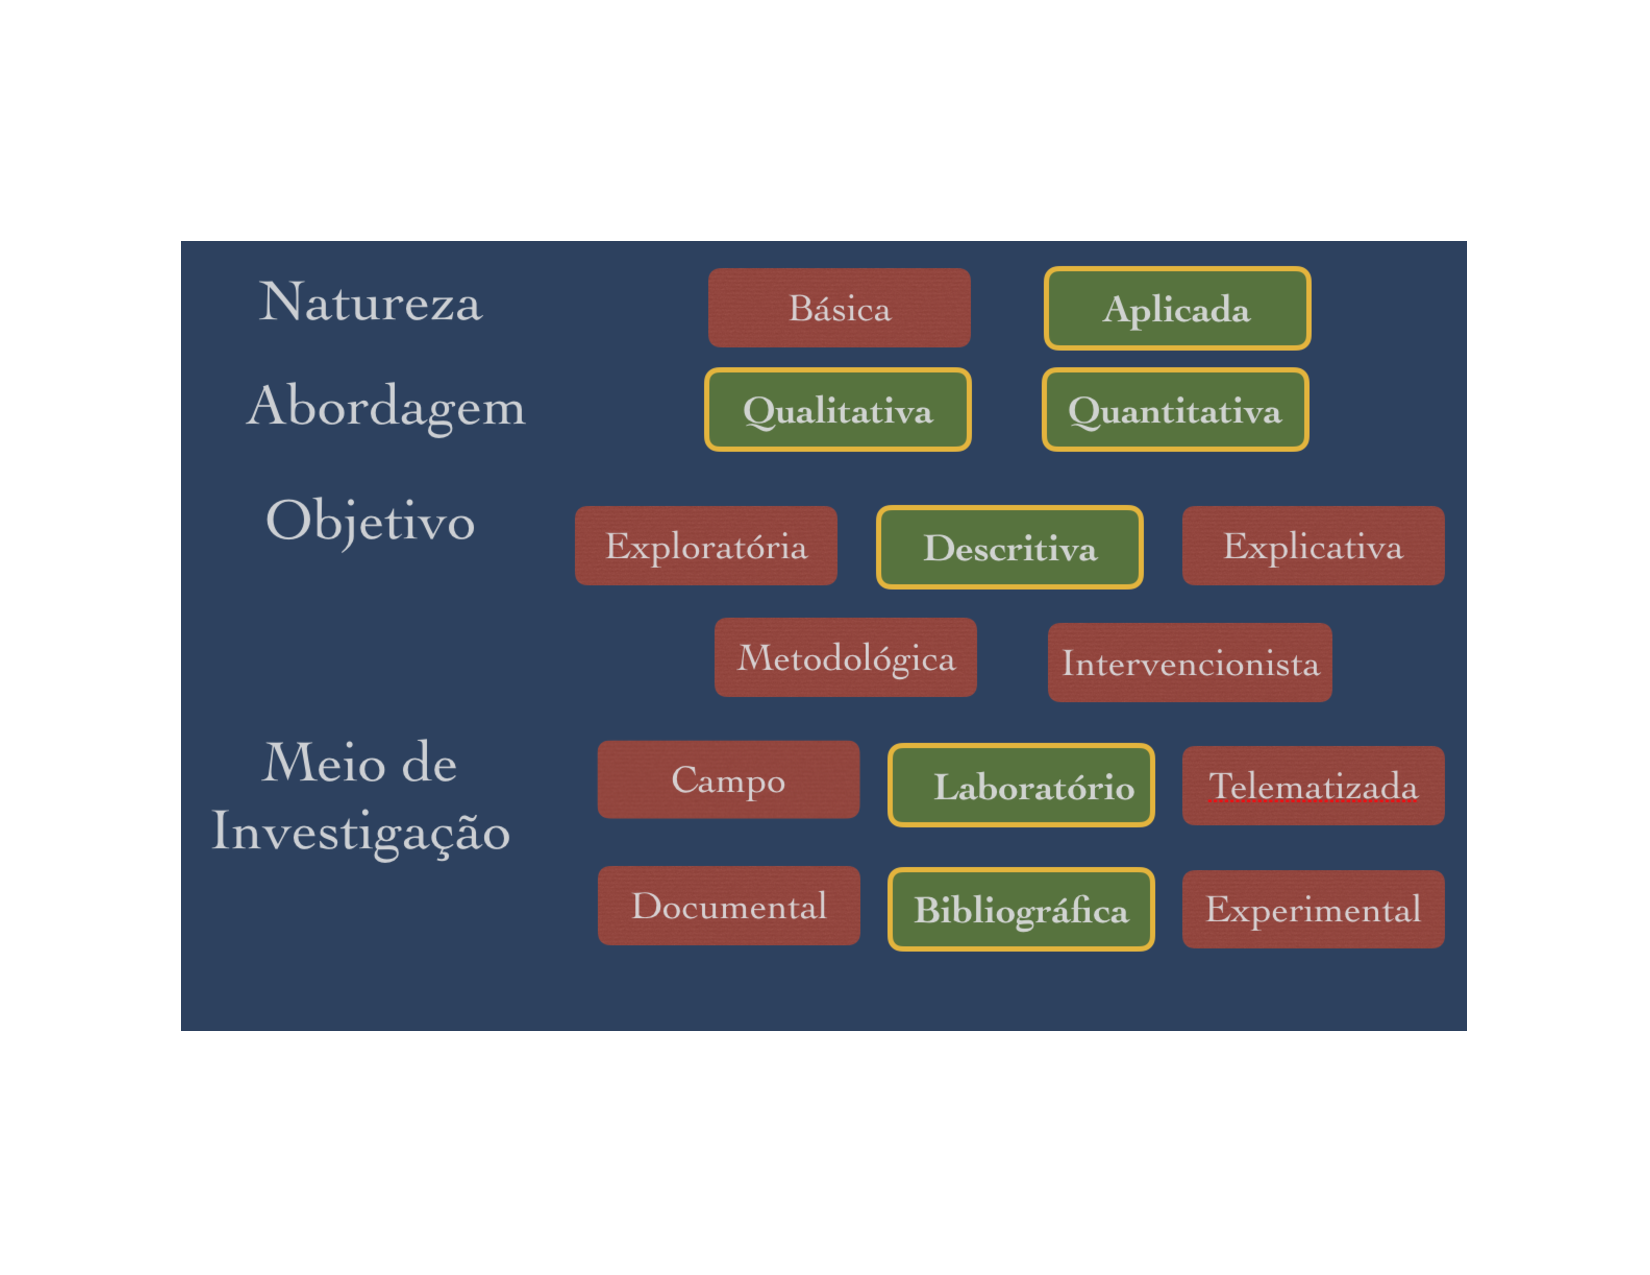
\includegraphics[scale=0.50]{metodologia_pesquisa}
\caption{Seleção das Características Metodológicas. Fonte: \cite{moresi_metodologia_2003}}
\label{img:met_pesquisa}
\end{figure}

Este trabalho tem um caráter mais voltado para uma pesquisa aplicada por envolver características espécificas na contratação de software do governo brasileiro. Outra característica que determina este trabalho como uma pesquisa aplicada é a natureza do trabalho estar voltado para o uso nas áreas de TI dentro dos orgãos públicos.

Segundo \cite{tatiana_denise} a pesquisa qualitativa é mais voltada para aspectos da realidade que não podem ser quantificados, mantendo o foco na compreensão. Neste aspecto o trabalho apresenta características qualitativas uma vez que a construção da solução é feita de maneira dinâmica se adaptando as necessidades do usuário. Segundo as autoras outra característica inerente a este tipo de pesquisa é a observação do mundo social ao mundo natural, está característica se apresenta de maneira muito forte quando propor a solução foi adotado um conjunto de métricas que são utilizadas no mercado ao invés de outros conjuntos apresentados por outros autores. 

Para Gil \cite{gil_como_2002} a pesquisa descritiva é focada em analisar características de uma população, fenômeno ou a relação entre as váriaveis as que compõem. Ests tipo de pesquisa não visa explicar os fenômenos que está descrevendo (apesar que a explicação para o fenômeno possa servir como base) \cite{moresi_metodologia_2003}. Este trabalho apresenta o caráter descritivo ao se tratar da natureza das contratações de software para orgão brasileiros, ou quando se fala de um processo de manutenção de software.

Outra característica deste trabalho é o fato de se tratar de uma pesquisa 	de laboratório. Moresi destaca que a pesquisa de laboratório atua em um ambiente controlavel em que o pesquisador não tem a possibilidade de atuar em campo. Neste trabalho a pesquisa em campo se torna algo complicado pois é difícil de se conseguir acesso a orgãos públicos para instalação de uma ferramenta que ainda está em desenvolvimento. Por este motivo a pesquisa em laboratório é a mais adequada, em que são recriados as mesmas condições de uma situação em campo, porém com o controle de um ambiente simulado.

\subsection{Plano Metodológico}
\label{plano_metodologico}
O plano metodológico consiste em duas fases: Iniciação e Execução. Durante o TCC1 será implementado somente a primeira fase e a fase de Execução será implementadaß no TCC2. A primeira fase (imagem \ref{img:iniciacao}) possui seis atividades principais, são elas: Definir Tema, Validar o Escopo, Elaborar um roteiro de pesquisa, Pesquisar Referencias, Refinar Pesquisa e Catalogar material encontrado.
\graphicspath{{figuras/}}
\begin{figure}[h]
\centering
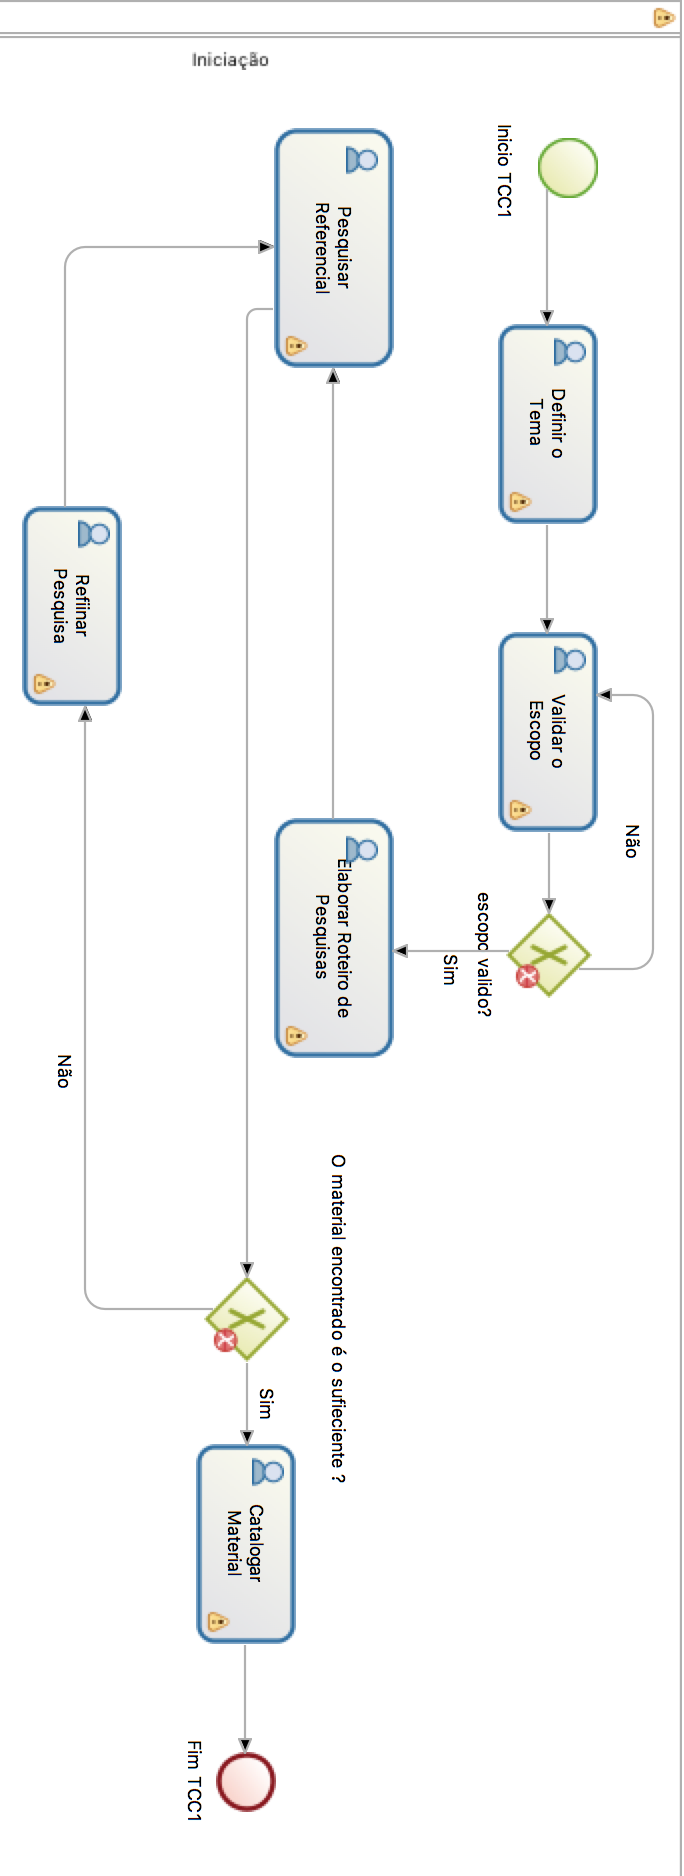
\includegraphics[scale=0.40]{iniciacao}
\caption{Modelagem da Fase de Iniciação}
\label{img:iniciacao}
\end{figure}

A Primeira atividade de Definir um Tema acontece logo no início do processo para que seja possível estabelecer em que área e sobre o que será discutido no trabalho. Uma vez escolhido o tema é preciso definir o escopo do trabalho para que seja possível definir quais são as fronteiras impostas tanto pelo tempo, pois é um prazo curto, quanto pelo conhecimento. Uma vez definido tema o escopo é validado juntamente com os professores orientadores para que haja um acordo entre aluno e orientador sobre o que será trabalhado.

Com o tema definido é necessario Elaboar um Roteiro de Pesquisa  que consiste em encontrar a melhor string de busca para o tema. Neste projeto as strings foram montadas de acordo com o tema da pesquisa então não houve uma string geral que perpassa-se por todo o conhecimentodo trabalho. Essa escolha se deu pelo fato de que este trabalho passou por adaptações até que se chegasse ao trabalho que é hoje, então as primeiras strings eram feitas com conceitos chaves e já definidos, com o decorrer o trabalho foi ganhando um escopo mais conciso.

A atividade de Elaborar Referências e Refinar Pesquisa envolviam o processo de aplicar a string nos motores de busca selecionados, que no caso foram Google Scholar e Periódicos Capes. Uma vez aplicada a string o primeiro ponto a ser observado nos resultados era o título do material, caso o titúlo tivesse alguma relação com o tema pesquisado o artigo era separado (esse processo era válido somente para as duas primeiras páginas de resultados). Com os artigos separados lia-se os tópicos do artigo e havendo um conteúdo referente à pesquisa lia-se o artigo completo. Caso o  material encontrado fosse insuficiente para o assunto gerava-se uma nova string de busca com termos aproximados ou mais refinados e o processo se repetia.

Catalogar material é uma atividade focada em guardar os materiais encontrados colocando uma tag referente ao tema a que o artigo se refere e uma breve descrição sobre o que era mais importante. Esse armazenamento é feito através de duas ferramentas de gerenciamento bibliográfico, o Zotero e o BibDesk. O Zotero foi utilizado para fazer a catalogação online dos materiais e gerar a bibliografia encontrada de cada material como mostra na figura \ref{img:zotero}.
\begin{itemize}
\item Área 1 - Categorização por pastas dos artigos encontrados.
\item Área 2 - Artigos referentes à categoria seleciona. Dentro de cada artigo é possível encontrar a nota e um link para leitura do artigo selecionado.
\item Área 3 - Informações do artigo selecionado.
\item Área 4 - Tags referentes ao artigo.
\end{itemize}
Uma vez que o material era catalogado no Zotero ele era exportado para o Bibdeks por ter uma melhor integração com o Latex.
\graphicspath{{figuras/}}
\begin{figure}[h]
\centering
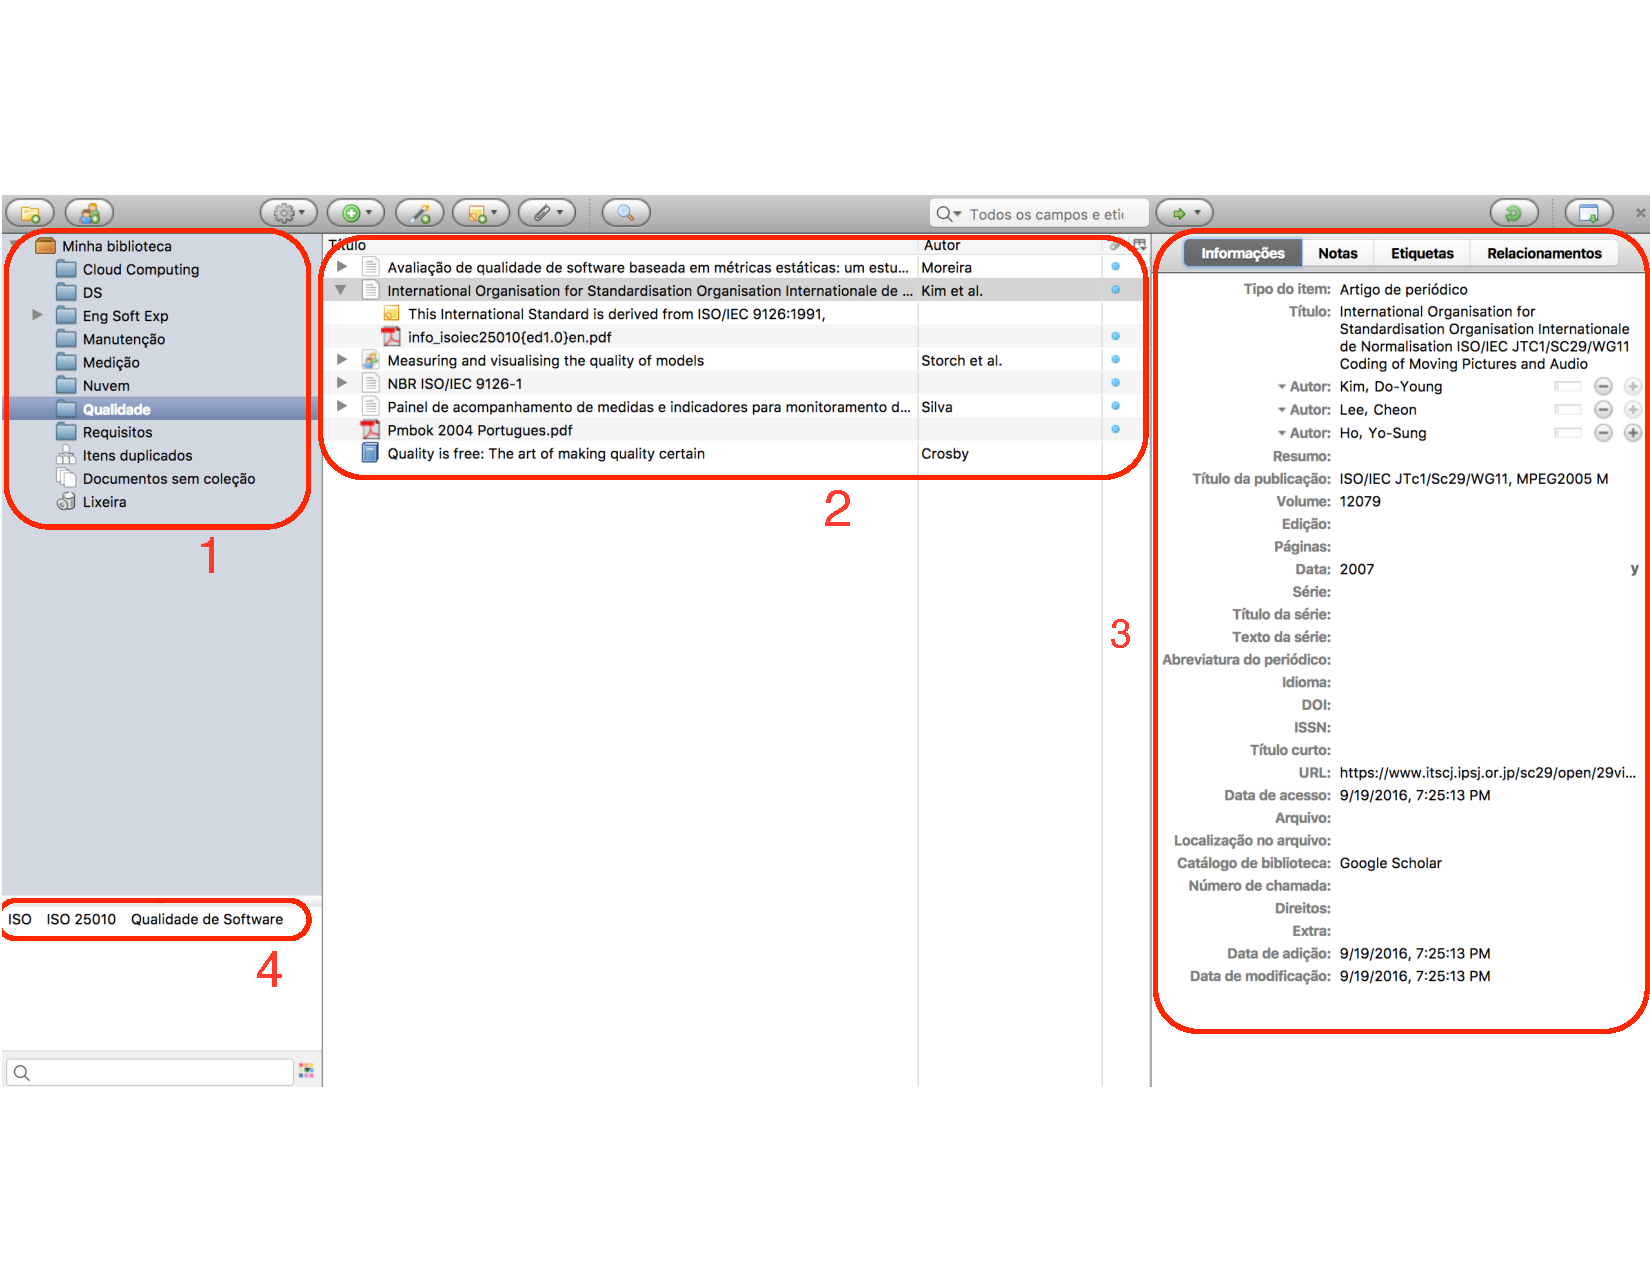
\includegraphics[scale=0.50]{zotero_edit2}
\caption{\textit{Screenshot} do Zotero contendo as categorias dos materiais pesquisados, suas \textit{tags} e anotações}
\label{img:zotero}
\end{figure}
Após catalogar o material encontrado finaliza-se a fase de iniciação do projeto. Esta fase deixa como insumo para a próxima fase: o trabalho produzido até então e decisões de escopo e cenários de uso que serão implentados na fase de elaboração. 

A Fase de Execução (figura \ref{img:execucao}) possui sete atividades sendo que a atividade de Documentação ocorre durante todo o processo. O objetivo desta fase é implementar o que foi decidido na fase de iniciação. A primeira atividade da segunda fase é Analisar o Ambiente. Por se tratar de um ambiente simulado é necessário que se estude quais são as melhores ferramentas e configuração entre elas para que se reproduza um ambiente mais próximo do real possível. Uma vez definido é necessário Configurar este ambiente o que deve ser feito seguindo as configurações de um ambiente real.
\graphicspath{{figuras/}}
\begin{figure}[h]
\centering
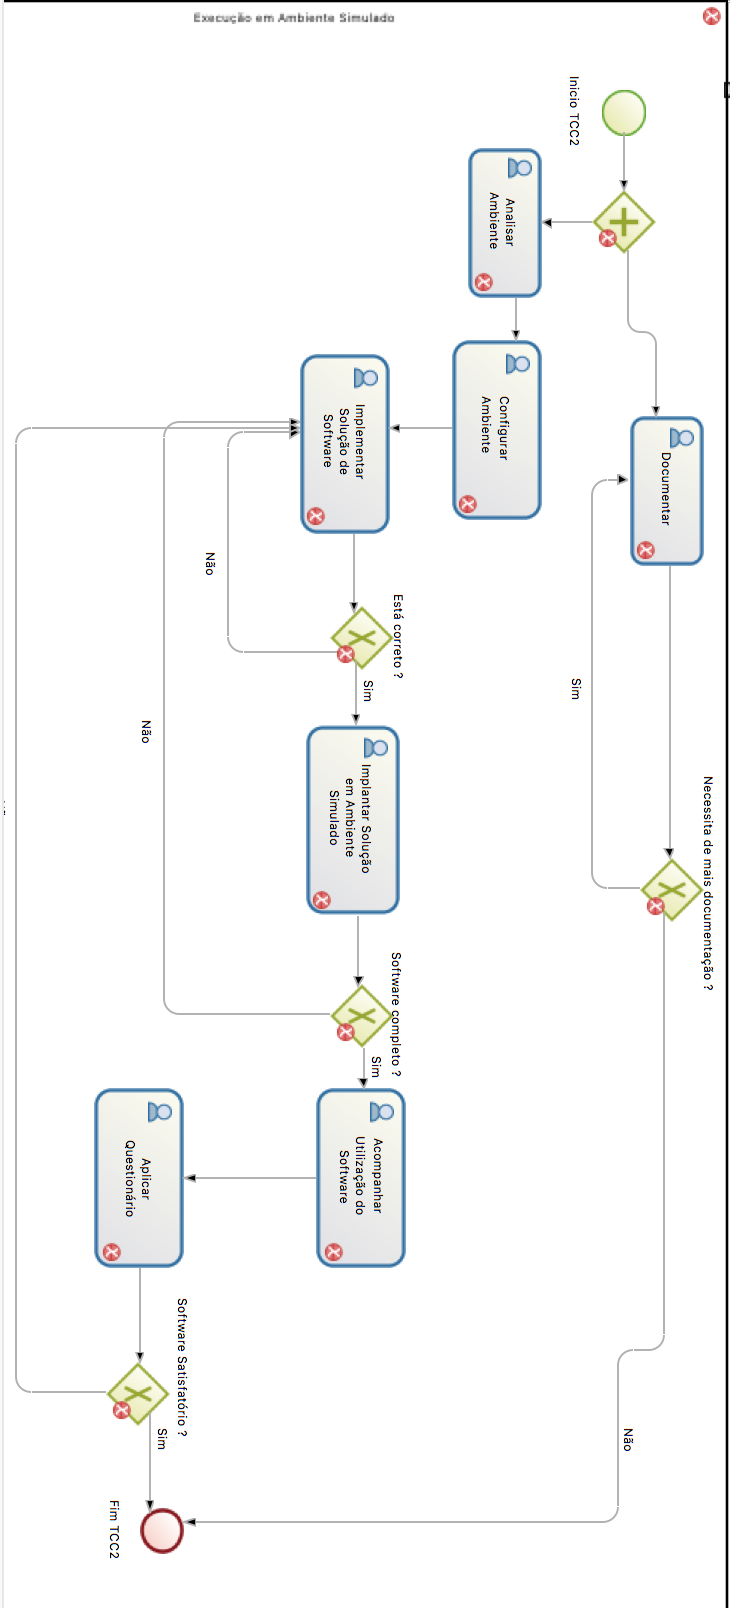
\includegraphics[scale=0.40]{execucao}
\caption{Modelagem da Fase de Execução}
\label{img:execucao}
\end{figure}

A terceira atividade é Implementar a Solução. Está atividade segue os principios de desenvolvimento ágil para construção de soluções em software, para isso seu desenvolvimento é feito de maneira iterativa incremental de forma que a cada iteração haja um implemento funcional de software. Ao fim de cada iteração se o software produzido estiver funcionando e testado ele é colocado no ambiente simulado para que se possa acompanhar o seu funcionamento enquanto em um ambiente "produção".

Uma vez que a solução em software esteja completa ela é disponibilizada para um conjunto de utilizadores que irão testar a solução e documentar as suas impressões quanto a utilização da solução. A última atividade desta fase é relacionada ao questionário que é aplicado aos utilizadores da ferramenta para que se possa avaliar o quão efetiva foi a solução. 

Com a Fase de Execução finalizada o processo se encerra. Nesta segunda fase os principais artefatos são: a solução funcionando e um refinamento do documento entregue na primeira fase. A figura \ref{Rotulo} apresenta uma visão geral do processo que será aplicado neste trabalho.
\graphicspath{{figuras/}}
\begin{figure}
\centering
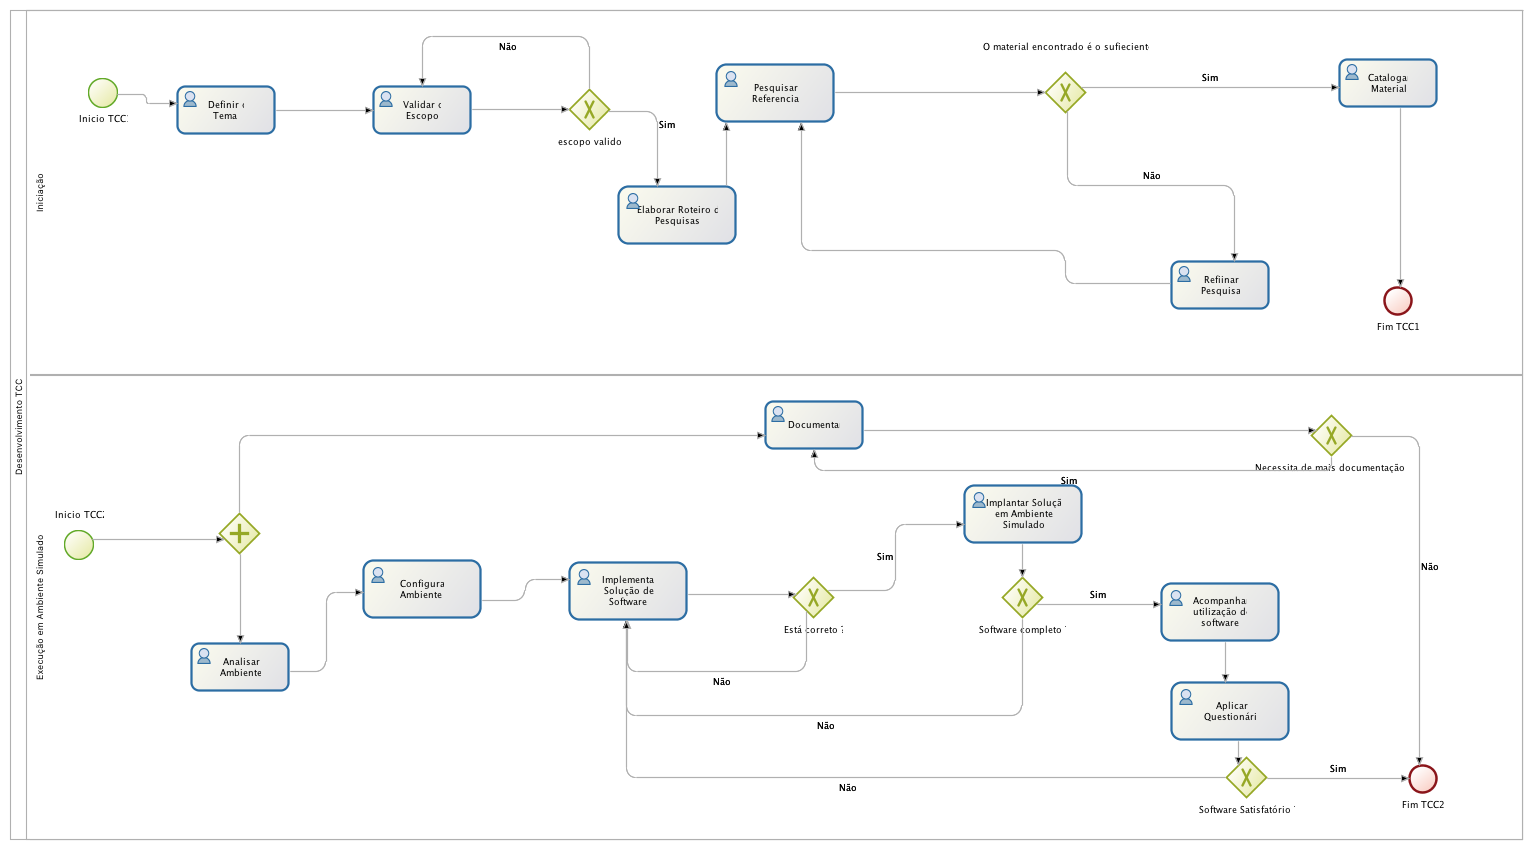
\includegraphics[scale=0.40]{TCCMetodologia}
\caption{Plano de Pesquisa}
\label{Rotulo}
\end{figure}

\section{Metodologia de Desenvolvimento}
\label{met_desenvolvimento}
O dashboard será criado utilizando de uma adaptação da metodologia de desenvolvimento Scrum. O Scrum é uma metodologia de desenvolvimento de software baseada em princípios de desenvolvimento ágil. As metodologias ágeis tem sido muito utilizadas em projetos 	com times pequenos, curto prazo de entrega do software e os requisitos são constantemente alterados \cite{lopez-martinez_problems_2016}. Como o Scrum é um modelo de desenvolvimento iterativo e incremental ele quebra o projeto de desenvolvimento em pequenas entregas chamadas de \textit{sprints} que podem ser associados a pequenos ciclos de desenvolvimento que duram entre duas a quatro semanas. As \textit{sprints} são consecutivas e nesse período algumas funcionalidades do sistema são implementadas e testadas \cite{pagotto_scrum_2016}. Na figura \ref{img:scrum} pode-se observar que o as funcionalidades desenvolvidas na \textit{sprint} advêm de um escopo definido no início do projeto chamado de \textit{product backlog} que é o conjunto de todas as funcionalidades do sistema, o conjunto de funcionalidades separadas para uma determinada \textit{sprint} é chamada de \textit{sprint backlog}\cite{sabbagh_scrum:_2014}.
\graphicspath{{figuras/}}
\begin{figure}[h]
\centering
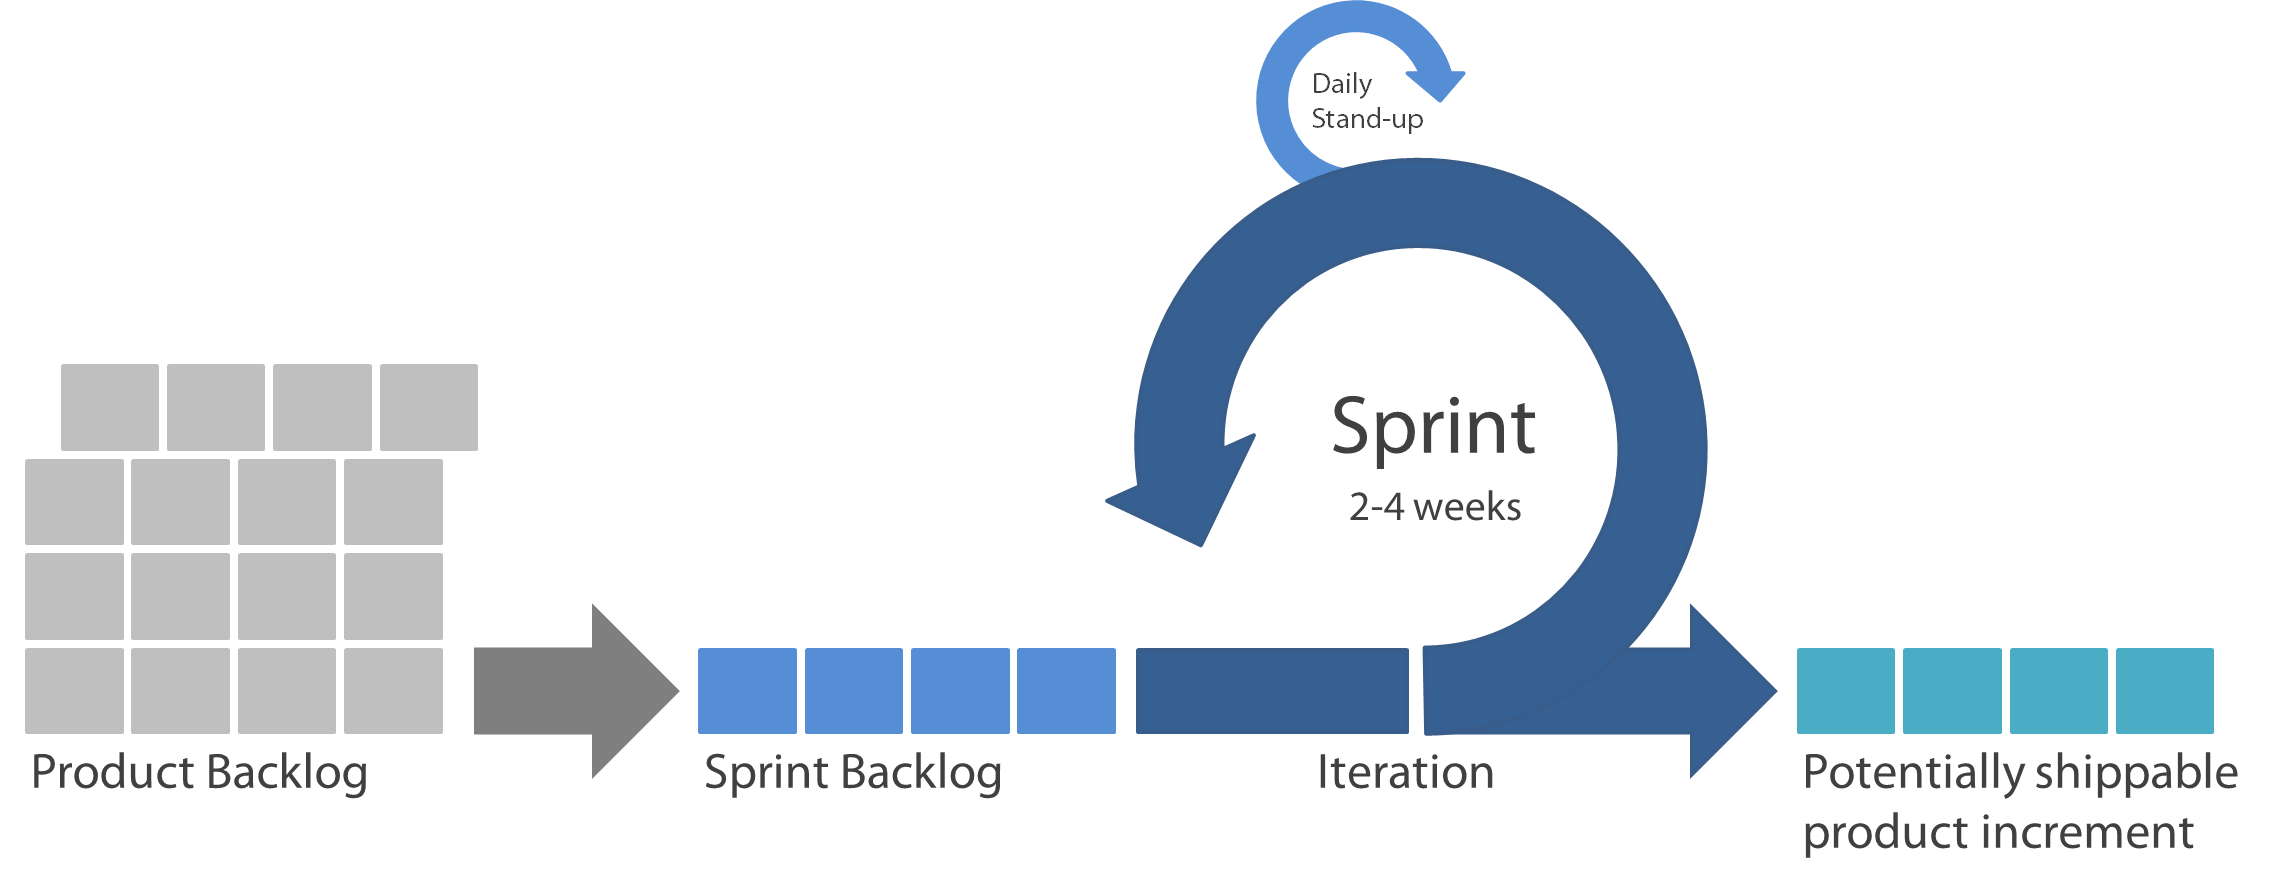
\includegraphics[scale=0.40]{scrum}
\caption{Ciclo de Desenvolvimento do Scrum}
\label{img:scrum}
\end{figure}

Os principais conceitos que foram utilizados da metodologia foram:
\begin{itemize}
\item \textit{\textbf{Product Backlog}}: Lista de atividades que representam as funcionalidades que serão construidas no projeto. O \textit{Product Owner} é quem escreve o \textit{product backlog}, essas atividades são mutáveis ao decorrer do projeto, pois a equipe de desenvolvimento acaba conhecendo mais do produto \cite{sabbagh_scrum:_2014}.
\item \textit{\textbf{Sprint}}: Ciclo de desenvolvimento com prazo definido em que são desenvolvidas as atividades do projeto. Neste trabalho definiu-se como sendo 15 dias o período referente a uma \textit{Sprint}
\item \textit{\textbf{Sprint Backlog}}: Atividades referentes à uma determinada \textit{Sprint} na qual a equipe de desenvolvimento se compromete a entregar. Estas atividades são retiradas do \textit{product backlog} \cite{mahnic_case_2011}.
\item \textbf{História do Usuário}: Descrição do ponto de vista do usuário sobre uma funcionalidade do produto. Este artefato é composto do que é conhecido como 3C's, Cartão, Conversa e Confirmação. O cartão é referente ao fato de se documentar a conversa em um cartão, este sendo acessível a todo o time de desenvolvimento. A conversa é uma breve descrição da funcionalidade sob o olhar do usuário, um exemplo pode ser observado na figura \ref{img:us}. E a confirmação ou critérios de aceitação é um \textit{checklist} abordando o que deve ser verificado para que a história seja dada como concluida.
\graphicspath{{figuras/}}
\begin{figure}[h]
\centering
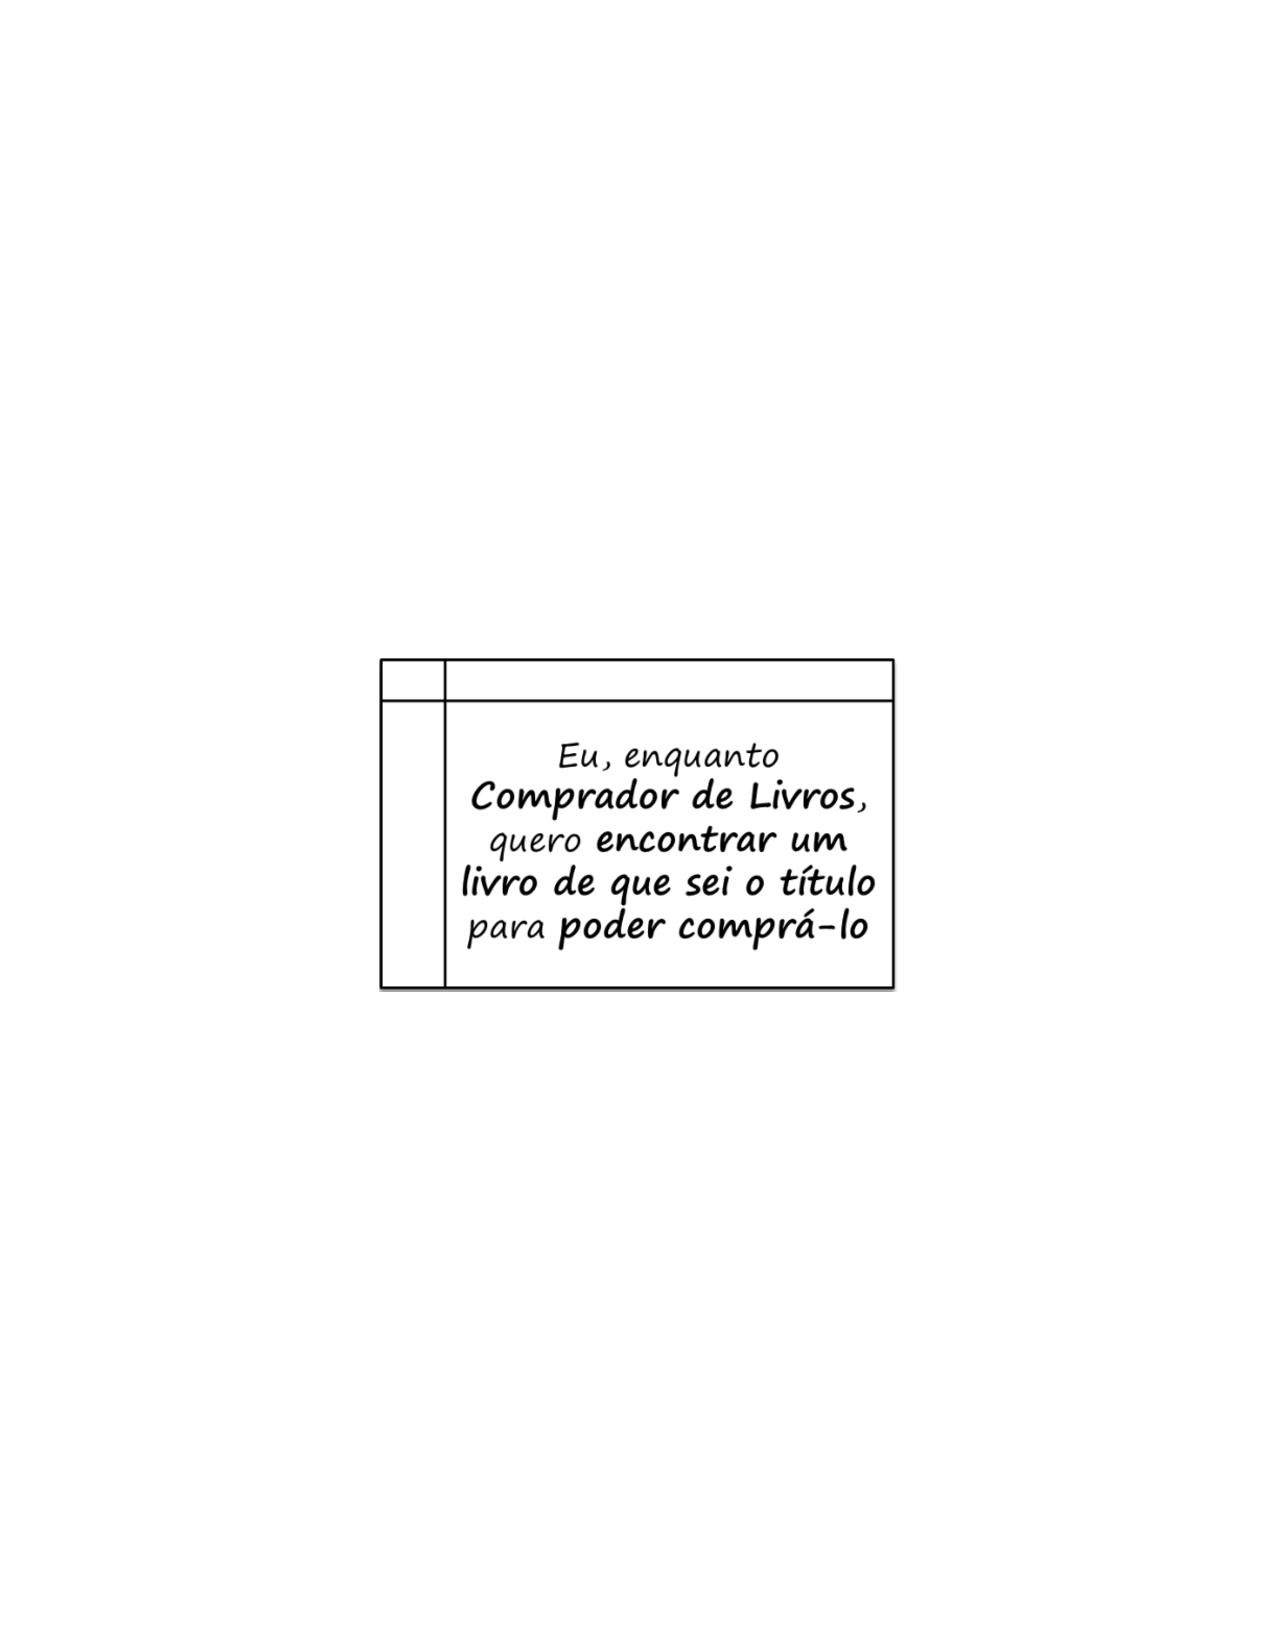
\includegraphics[scale=0.80]{US}
\caption{Exemplo de História de Usuário. Fonte: \cite{sabbagh_scrum:_2014}}
\label{img:us}
\end{figure}
\item \textit{\textbf{Story Point}}:Unidade relativa que caracteriza o esforço da equipe de desenvolvimento para finalizar uma atividade. A escala utilizada é definida pela equipe de desenvolvimento, neste trabalho será utilizado a escala de Fibonacci (1,2,3,5,8,13, ...). 
\item \textit{\textbf{Kanban}}: Forma de visualização de atividades muito utilizadas com cartões que são movimentados em um quadro determinando o status da atividade como mostra a figura \ref{img:kanban}.
\graphicspath{{figuras/}}
\begin{figure}[h]
\centering
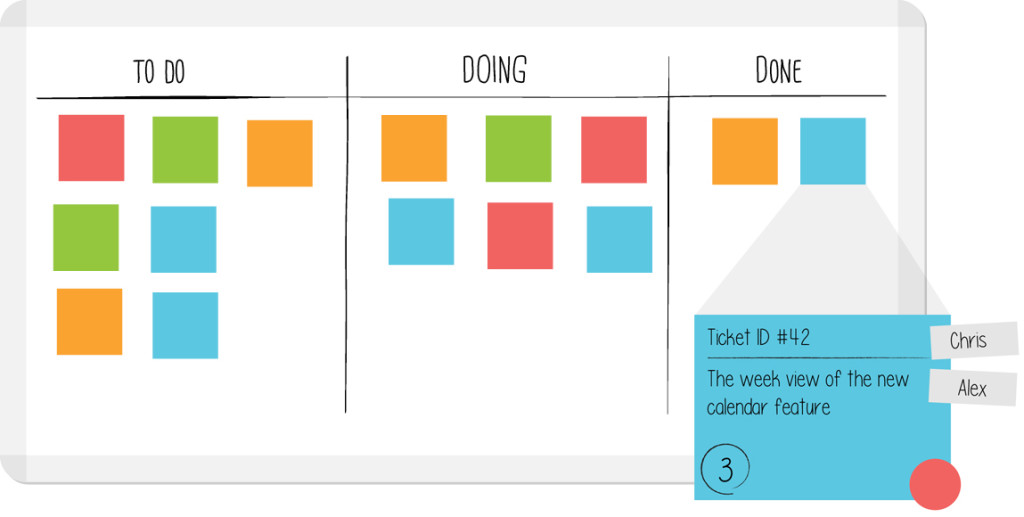
\includegraphics[scale=0.40]{kanban}
\caption{Exemplo de \textit{Kanban}}
\label{img:kanban}
\end{figure}

\end{itemize}
\section{Cronograma}
\label{cronograma}
Para que se possa ter uma visão mais abrangente da organização do trabalho foi criado um cronograma em que constam as atividades definidas no \ref{plano_metodologico}. Este cronograma serve como orientação ao desenvolvimento e planejamento do projeto contudo com o decorrer das atividades este artefato pode sofrer alterações. O cronograma foi dividido em duas tabelas referentes às atividades do TCC1 e TCC2.

\subsection{Cronograma TCC1}
A tabela \ref{cronograma_tcc1} apresenta um cronograma em relação as ativdades a serem desenvolvidas enquanto TCC1

\begin{table}[h]
\centering
\caption{Cronograma TCC1}
\label{cronograma_tcc1}
\begin{tabular}{lllll}
\textbf{Atividade}           & \textbf{Agosto} & \textbf{Setembro} & \textbf{Outubro} & \textbf{Novembro} \\ \hline
Definir Tema                 & X               &                   &                  &                   \\ \hline
Validar Escopo               & X               &                   &                  &                   \\ \hline
Elaborar Roteiro de Pesquisa &                 & X                 & X                &                   \\ \hline
Pesquisar Referência         &                 &                   & X                & X                 \\ \hline
Refinar Pesquisa             &                 &                   & X                & X                 \\ \hline
Catalogar Material           &                 &                   &                  & X                 \\ \hline
\end{tabular}
\end{table}

\subsection{Cronograma TCC2}
A tabela \ref{cronograma_tcc2} apresenta um cronograma em relação as ativdades a serem desenvolvidas enquanto TCC2
\begin{table}[h]
\centering
\caption{Cronograma TCC2}
\label{cronograma_tcc2}
\begin{tabular}{lllll}
\textbf{Atividade}                     & \textbf{Março} & \textbf{Abril} & \textbf{Maio} & \textbf{Junho} \\ \hline
Documentar                             & X              & X              & X             & X              \\ \hline
Analisar Ambiente                      & X              &                &               &                \\ \hline
Configurar Ambiente                    & X              &                &               &                \\ \hline
Implementar Solução de Software        &                & X              & X             &                \\ \hline
Implantar Solução em Ambiente Simulado &                & X              & X             &                \\ \hline
Acompanhar Utilização do Software      &                &                &               & X              \\ \hline
Aplicar Questionário                   &                &                &               & X              \\ \hline
\end{tabular}
\end{table}

\section{Resumo do Capítulo}
A pesquisa pode ser classificada de diversas formas, neste a projeto a natureza da pesquisa pode ser classificada como Aplicada devido ao uso nas áreas de TI. Quanto a sua abordagem ela é do tipo Qualitativa pois a forma de se analisar e coletar os dados é feito de maneira empírica e através da observação. Sobre o seu objetivo essa pesquisa tem um caráter Descritivo pois ela observa fatores de um grupo e os descreve neste caso a maneira como funciona a aquisição de software por parte da APF. E por último quanto ao meio de investigação que Laboratorial pois todo o desenvolvimento da pesquisa é feita em um ambiente controlado e não em campo.
Quanto a metodologia de desenvolvimento optou-se por uma adaptação da metodologia Scrum, isto se deu pelo fato de que o framework da metodologia é adaptável para times de desenvolvimento pequenos e com entregas de software em curtos períodos de tempo.
